\documentclass{paper}

\title{\bf{Becoming the King of Hearthstone \\ Battlegrounds with Reinforcement Learning}}
% \title{\bf{A Computational Analysis of Climate Change Sentiment on Social Media using Deep Neural Networks and SOTA Transformers for Multi-Class Tweet Classification, as a Heuristical Proxy for Context
% }}
\author{Shon Verch and Grace Lin}
\date{}

% Font
\usepackage[scaled=0.8]{FiraMono}

% Graphics
\usepackage{xcolor}
\usepackage{placeins}
\usepackage{graphics}
\usepackage{tikz, ifthen, fp, calc}
\usepackage{pgfplots, pgfplotstable}
\usetikzlibrary{patterns, positioning}
\usetikzlibrary{arrows, decorations.markings}
\usepgfplotslibrary{fillbetween}
\usepgfplotslibrary{groupplots}

% Math imports
\usepackage{bm}
\usepackage{amsthm}
\newtheorem{definition}{Definition}
% Use bold instead of vector arrow
\let\vec\mathbf
\newcommand{\mat}[1]{\bm{#1}}

% Data tables for graphs
\include{graphs}
% Subfigures
\usepackage{caption}
\usepackage{subcaption}

% Tables
\usepackage{booktabs}
\usepackage{tabularx}
\usepackage{makecell}
 \newcolumntype{P}{>{\raggedleft\arraybackslash}p{.2in}}
%dashed line
\usepackage{array}
\usepackage{arydshln}
\setlength\dashlinedash{0.2pt}
\setlength\dashlinegap{1.5pt}
\setlength\arrayrulewidth{0.3pt}

\newcommand\Tstrut{\rule{0pt}{2.6ex}}         % = `top' strut
\newcommand\Bstrut{\rule[-0.9ex]{0pt}{0pt}}   % = `bottom' strut

% BibTeX
\usepackage{url}
\usepackage[hidelinks]{hyperref}
\usepackage{csquotes}
\usepackage[block=ragged,backend=bibtex,maxbibnames=99, sortcites]{biblatex}
\addbibresource{references.bib}

% Convenience Macros
\newcommand{\inlineSection}[1]{\vspace{0.5em}\noindent\textbf{#1.}~}
\newcommand{\targetWord}[1]{\underline{\textbf{#1}}}

\DeclareMathOperator*{\argmax}{arg\,max}
\DeclareMathOperator*{\argmin}{arg\,min}

\begin{document}

\maketitle

%%%%%%%%% ABSTRACT
\section*{Abstract}
With the increasing popularity in digital card strategy games, there is serious value in researching the ability for autonomous play in such genres. In this paper, we aim to create an AI agent for Hearthstone Battlegrounds that uses the Monte-Carlo Tree Search algorithm. We then compare it to other different AI, to assess its performance. We find that our algorithm, a variant of MCTS modified to handle imperfect information and randomness, is able to consistently outperform a random player. Our results act as a proof-of-concept for AI research in Hearthstone Battlegrounds.

%%%%%%%%% BODY TEXT
\section{Introduction}
Hearthstone Battlegrounds is the game mode of the popular turn-based collectible card game Hearthstone, where eight players face off in different 1v1 battles, with the goal to be the last person standing \cite{blizzardentertainment2019}. Unlike other card games however, players are unable to choose specific moves for their cards; but instead combat between cards happens automatically once the battle starts, and continues until a victor is decided. 

\subsection{A Tour of Hearthstone Battlegrounds}
Since our project revolves around a fairly complex domain, let us first explain the main details of the game. 
\subsubsection{Recruitment Phase}
The recruitment phase is where the game initially starts. Each round, the player can make decisions for their game board, limited to the amount of coins the player has to spend for each round. 

\inlineSection{I. Recruitment}
At the beginning of every round, the player visits Bob's cavern, where minions can be purchased from the tavern keep Bob. Each minion will cost 3 Gold, and can be placed on your board as game pieces. The player can upgrade their "Tavern Tier" if they have the gold necessary, which allows them access to buy higher-tier and better minions \cite{battlegrounds2019}. The money for each round does not transfer to the next round, and all enhancements are permanent. 

\inlineSection{II.  Triple Cards}
When a player has two minions of a kind, purchasing a third one will combine the three into a single golden, Triple Card. This created card is an enhanced version of the minion, with significant increase in stats and effects.

\inlineSection{III. Additional Options}
When one wishes, minions can also be sold back to Bob, for 1 coin each. On top of that, there are configurations for the shop, including refreshing the store for 1 gold in order to randomize the shop, or the option to freeze your shop for next round, meaning the minions for sale currently will be kept for next round, instead of the game randomizing another pool of minions to buy\cite{battlegrounds2019}. Additionally, minions can be rearranged on the board, which is important in determining the order in which the minions attack.
\begin{figure*}[ht]
    \centering
    \begin{tikzpicture}[
        x=1mm, y=1mm,
    ]
    \node[anchor=south west=inner sep=0pt] (fig1) at (0, 0) {\fbox{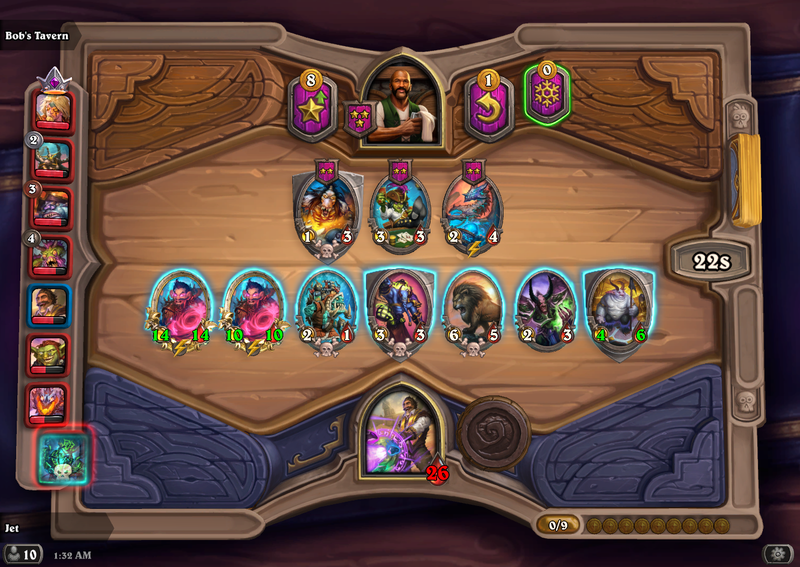
\includegraphics[width=0.8\textwidth]{figs/hsbg_recruitment_phase.png}}};
    
    % Rankings
    \filldraw[draw=red!50!white,fill=red!20!white,opacity=1, fill opacity=0.25] (6,16) rectangle (16,95);
    
    \filldraw[draw=red!50!white,fill=red!20!white,] (6, 95) rectangle (6+5,95-5) node[color=black,opacity=1,pos=0.5] {1};
    
    % Cheer!
    \filldraw[draw=red!50!white,fill=red!20!white,opacity=1, fill opacity=0.25] (50.5,77) rectangle (65.5,92);
    
    \filldraw[draw=red!50!white,fill=red!20!white,] (50.5, 92) rectangle (50.5+5,92-5) node[color=black,opacity=1,pos=0.5] {2};
    
    % Refresh!
    \filldraw[draw=red!50!white,fill=red!20!white,opacity=1, fill opacity=0.25] (83,77) rectangle (96,92);
    
    \filldraw[draw=red!50!white,fill=red!20!white,] (83, 92) rectangle (83+5,92-5) node[color=black,opacity=1,pos=0.5] {3};
    
    % Frozen!
    \filldraw[draw=red!50!white,fill=red!20!white,opacity=1, fill opacity=0.25] (95,80) rectangle (105,93);
    
    \filldraw[draw=red!50!white,fill=red!20!white,] (95, 93) rectangle (95+5,93-5) node[color=black,opacity=1,pos=0.5] {4};
    
    % Gold!
    \filldraw[draw=red!50!white,fill=red!20!white,opacity=1, fill opacity=0.25] (97,7.5) rectangle (137,12.5);
    
    \filldraw[draw=red!50!white,fill=red!20!white,] (137, 7.5) rectangle (137-5,12.5) node[color=black,opacity=1,pos=0.5] {5};
    
    \end{tikzpicture}
    \caption{Elements of the Hearthstone game board during the recruitment phase: (1) player rankings, (2) ``cheer'' button (upgrade Bob's Tavern), (3) swap available minions for a new selection, (4) freeze the selection of minions until the next Recruit phase, and (5) the amount of Gold available \cite{battlegrounds2019}.}
    \label{fig:embedding_projector}
\end{figure*}

\subsubsection{Combat Phase}
The combat phase is where players face off against others, and play against their boards. For Battlegrounds, this involves no decisions to be made on the player's part. Certain moves are randomized, and all attacks, buffs, and effects happen automatically. Yet, despite this, the combat phase is \textit{essential} in determining the outcome of the game since the health of the hero is the sole determining factor for whether a player stays in the game. In this section, we provide a brief summary of the components of the combat phase, and enumerate through the possible actions.
%Since this is an 8  player game with eliminations, if there is an uneven number of players alive, one player will face off against an AI, which takes the board of a previously defeated player. 

\inlineSection{I. Attack}
To  begin, 2 players are randomly put against each other on the field. The player with the greater number of minions starts first (or randomized when minion counts equal). Minions attack automatically starting from the leftmost, and all attacks are randomized with consideration to special effects and abilities. The attack ends when one player's minions are destroyed \cite{battlegrounds2019}.

\inlineSection{II. Damage}
After the attack phase is over, the player with surviving minions (if any) deals damage to their opponent Hero. The damage is given by
$$
\textit{Damage Dealt} = \textit{Tavern Tier} + \textit{Tier of Each Surviving Minion}.
$$
If the game ended in a draw, no damage is dealt.  Each hero starts off with 40 health points, and a player is out of the game if the damage dealt to  the player Hero results in their health dropping below 0. At the end of the combat phase, any minion that was killed is brought back to life, and each player's board is restored to its state before combat, with the exception to any permanent effects that may have been applied during the combat phase, and the Hero's health.


\medskip

Battlegrounds and the entirety of the genre, including other popular games such as DOTA Autochess and Team-fights Tactics have garnered a lot of attention as of late, and professional play has become increasingly popular. With over 33 million people playing  every month, competitive scenes are popping up everywhere, meaning the ability to excel in these games has exponentially grown in value \cite{stavropoulos_2019}. In that respect, there is serious value in researching autonomous play of Hearthstone Battlegrounds. Besides the mere intrinsic and entertainment value of an AI that plays Battlegrounds, the popularity of the game makes it a demanding challenging for AI research. And, AI agents have the potential to change the landscape of gaming. From a developer perspective, an AI agent can be leveraged for fast iteration the game design process, whereby well-trained agents play test the game, and provide feedback to designers. Due to the sheer computational prowess of artificial intelligence, AI agents can traverse a search space with great speed. All the while, an AI agent can discover new strategies (ones not even thought by the designers!), and has the potential to completely alter the most popular strategies available. This is not just valuable for a game developer, but also beneficial for the player community as a whole. 

Of course, though the algorithm proposed in this paper may not achieve that level of success, at very least, we provide the agent as an initiative for further research in this problem domain.\footnote{Perhaps it can even assist us in climbing the ranks of Battlegrounds!}

In this paper, we investigate the context for researching AI in Hearthstone, and propose our own methodology for a Battlegrounds agent. We ask the question \textbf{``How can we create an AI agent to play Hearthstone Battlegrounds, and how can we evaluate its performance?''} Of course, there's much potential for the abilities of video game AIs, as shown from OpenAI's DOTA 2 bot that beat 99.4\% of players \cite{wiggers_2019}. However, the process to creating an AI, let alone a good AI, is a very difficult task. As we mentioned, Hearthstone Battlegrounds is a complex domain, and simulating a game is challenging due to many different factors. 


\subsection{The Complexity of the Domain}
Hearthstone and other games categorized under the ``Auotchess'' game genre (named after the first game of its kind, DOTA Autochess) %citation
often have various factors that make creating an AI difficult.

\inlineSection{Partially Observable State Space} At any given time in the game, there is \textit{critical} information hidden from the player, making assessments of future game states only plausible realities. For example, each player visits Bob's Tavern separately, meaning the minions each player bought and own are not disclosed, until the Combat Phase is reached. Even then, the exact state of the enemy board is only precisely known for exactly one turn---the player may always add or remove minions from its board, and so there is no guarantee that the enemy board hasn't changed.\footnote{And we can bet that it will change!} Thus, this information is still largely hidden to the player. 

\inlineSection{The Aspect of Randomness} Due to majority of the game being automated, many choices are decided arbitrarily, meaning the state space is never fully deterministic. In the combat phase, all attacks are randomly chosen, and the outcome of the game is never entirely certain. The opponent each player is up against is also entirely randomized, and thus the outcomes and decisions of other players and their matches---which the the player largely doesn't have a deciding factor in---will also affect the chances of overall victory. Bob's Tavern is a stochastic process; the recruits (i.e. minions available for purchase), minions on the board and in the hand, and other interaction elements are random variables. This means that the transition from one state to another is never fully predictable. For example, consider refreshing Bob's Tavern from a state $S_t$. This yields \textit{at most} $N_t\choose r_t$ new states, called transition states, where $N_t$ is the number of minions in the pool in state $S_t$ and $r_t$ is the number of recruits offered to the player. When the pool is full, this corresponds 134 available minions to choose from, and Bob's Tavern offers at most $7$ recruits (this happens in special circumstances due to card effects) \cite{battlegrounds2019}. This means that there are a whopping ${{134}\choose{7}}\approx  1.3125\times 10^{11}$ possible states following a fresh with a full minion pool and recruitment size.

Though, each transition state only differs slightly---in which recruits are available---each is nonetheless unique, and thus must be evaluated independently. It follows that Hearthstone Battlegrounds is immensely \textit{combinatorially complex}; a single game state has virtually uncountable successor states.

As yet another point of complexity, note that the minions offered to the player are constantly changing, and is also affected by random chance. Specifically, the minions that a player is offered by Bob's Tavern depends on what minions other players have in the game, and thus is subject to the pool of other players. This is due to the fact that the minions offered come from a pool of minions shared by \textit{all} of the players in the game. Thus, if another player buys a minion (unless that player is dead), another player will be less likely to be offered that minion. As a reference, the amount of copies of each minion is decided based on the Tavern Tier at which it is available for purchase. 

\begin{table}[h]
    \centering
    \begin{tabularx}{0.5\textwidth}{@{}XX@{}}\toprule
        \textbf{Tavern Tier} & \textbf{Copies of Each Minion}\\\midrule
       1 & 16 \\\hdashline
        2 & 25 \\\hdashline
        3 & 13 \\\hdashline
        4	& 11 \\\hdashline
        5	& 9 \\\hdashline
        6	& 7 \\\bottomrule
    \end{tabularx}
    \caption{Number of copies of each minion associated with each Tavern Tier \cite{battlegrounds2019}}
    \label{tab:copies_of_minions_by_tier}
\end{table}

\inlineSection{Dynamic Meta, and the Sizable Set of Cards}
One of the main reasons for the complexity of the domain is due to the sheer amount of cards within the game. In total, there are 134 unique minion types \cite{battlegrounds2019} in the game (or if the golden version of the minions are considered, 268), and each minion has a special unique ability. Additionally, each minion fit under many category (for example one minion could have a rarity of Legendary, a minion type of Demon, and a card class of Hunter), giving it a special affinity with other minions, and additional characteristics (Table \ref{tab:minion_count_by_type}) . For example, buying only a certain type of minion is considerably a good route to victory, as most minions have effects that require the existence of other minions of the same type. These different combination and synergies are not easily found through trial and error, but rather strategic planning and observations of the games themselves, making it more difficult for a trained AI to find through training. % TODO look over

\begin{table*}[t]
    \centering
    \begin{tabularx}{\textwidth}{@{}XXXXXXXXXX@{}}\toprule
        \textbf{Tier} & \textbf{Beast} &\textbf{ Demon }& \textbf{Dragon} & \textbf{Elemental} &\textbf{ Mech} & \textbf{Murloc} & \textbf{Pirate} & \textbf{Neutral} & \textbf{Total}\\\midrule
       1&2&2&2&2&2&3&2&2&17  \\\hdashline
        2&2&2&2&2&3&2&3&7&23 \\\hdashline
       3&3&2&3&3&5&2&3&6&27 \\\hdashline
       4&2&3&3&1&3&2&2&7&23 \\\hdashline
        5&2&3&2&1&2&1&3&8&22 \\\hdashline
        6&4&2&2&4&2&1&2&5&22 \\\hdashline
       \textbf{Total}&15&14&14&13&17&11&15&35&134 \\\bottomrule
    \end{tabularx}
    \caption{Minion Type Count by Tier Level}
    \label{tab:minion_count_by_type}
\end{table*}

Additionally, as of April 16th, 2021, the game is still in development, and consistently receiving updates. These updates include, but are not limited to, buffs or debuffs to minion stats, the removal or addition of certain cards, and the change of certain effects. What these changes could potentially mean is that a certain strategy that was valid previously would no longer be viable after a certain patch or change, making the decisions the AI make rather useless in the future. %TODO look over
However, even with all these setbacks and complexities, let us still see if it is feasible to create an AI agent for Battlegrounds, and answer our research question. 

\section{Datasets}

To facilitate a large-scale simulation of Hearthstone Battlegrounds, and to study the elements of the game, we desire a description of each game object. In this section, we outline the datasets acquired, along with the our approach to cleaning, filtering, and processing the data so that it can be used in simulation.

\inlineSection{HearthstoneJSON} Though there is no first-party dataset of Hearthstone cards, or any officially supported API for acquiring them, there still exist a myriad of  ways of extracting this data from the Hearthstone game client. One such method involves using internal data files used by the Hearthstone game engine. Specifically by parsing XML files containing internal representations of game objects. HearthstoneJSON is one such project that uses internal game client data to extract game objects. It is an initiative by a group called HearthSim---a collection of developers that work on libraries to interact with the game \cite{}. The project not only provides data dumps, but also a JSON API for interacting with the data. 

An archive of cards provided by the HearthstoneJSON project was accessed from the project \textit{GitHub} page \cite{hearthstonejson}. These archives contain all game objects used by the Hearthstone game client, however not all are required for Battlegrounds. To filter out which objects are needed for Battlegrounds, we scraped the Battlegrounds minion pool from the Hearthstone wiki. Then, we cross-referenced this data with the HearthstoneJSON archives to filter out all non-Battlegrounds related data. In total, after filtering and cleaning the data, we were left with every minion in the Battlegrounds pool as of \textit{Hearthstone Patch 20.0}, along with heroes, hero powers, and other miscellaneous objects.

\inlineSection{Hearthstone Wiki} The Hearthstone Wiki is a ``Hearthstone reference written and maintained by players'' of the game \cite{battlegrounds2019}. Though it is not affiliated with the game, it is a staple of the Hearthstone community, and as such a great hub for information related to Hearthstone. We leveraged Hearthstone wiki to synthesize \textit{two} datasets: the minion pool, and the ``wiki dumps.'' The former refers to a list of minions in Battlegrounds, sorted by tavern tier, which was used to augment the HearthstoneJSON data (as discussed above). This was necessary since the HearthstoneJSON data did not include information like minion tavern tier or golden copies, which is vital to Battlegrounds. On the other hand, the latter is a collection of \textit{all} text on the Hearthstone wiki. This was collected by using the MediaWiki API to traverse through all the pages and request the wiki-text in the \texttt{mediawiki} format. Then, the \texttt{pypandoc} library was used to convert the pages from \texttt{mediawiki} format to plain text.

\subsection{Cleaning the Hearthstone Wiki Dumps}
\label{sec:data_cleaning}

In its raw form, the scraped pages from the  Hearthstone Wiki are in the \texttt{mediawiki} format. This format makes heavy use of markup which is both bloated and not ideal for natural lagnauge processing. To reduce the size of the dataset and make it more conducive for tasks in NLP, we perform multiple cleaning steps. The pages are organised in a highly granulated structure. For each of these files, we apply a set of preprocessing operations.

First, we filter each page based on its size. We exclude pages with fewer than 10 tokens, and also remove any redirect pages (these are pages which simply redirect to another). We also discard irrelevant metadata (see the \texttt{clean} task in the \texttt{hearthstone\_wiki.py} script). 

% We only keep the following variables:
% \begin{itemize}
%     \item \texttt{created\_at}: the time the tweet was created.
%     \item \texttt{id}: the id of the tweet as assigned by Twitter.
%     \item \texttt{truncated}: boolean indicating whether the text was truncated.
%     \item \texttt{coordinates} (if not \texttt{null}): location of the client as a geoJSON object.
%     \item \texttt{place} (if not \texttt{null}): a \texttt{Place} object where the tweet is associated.
%     \item \texttt{quote\_count} (if not \texttt{null} or $0$): approximately how many times the tweet has been quoted.
%     \item \texttt{reply\_count} (if not \texttt{null} or $0$): number of times the tweet has been replied to.
%     \item \texttt{retweet\_count} (if not \texttt{null} or $0$): number of times the tweet has been retweeted.
%     \item \texttt{favorite\_count} (if not \texttt{null} or $0$): approximately how many times the tweet has been linked.
%     \item \texttt{lang}: the BCP 47 language id as corresponding the machine-detected language of the tweet, or \texttt{und} if no language could be detected.
% \end{itemize}

Stripping out unnecessary metadata significantly reduces the file size of the data set into manageable chunks. Next, from the converted wiki pages, we construct a corpus for training the word2vec models \cite{goldberg2014word2vec} (see the \texttt{make-corpus} task in the \texttt{hearthstone\_wiki.py} script). As our goal is to learn word embeddings, which will then be used to construct card embeddings, we simplify the data by removing Unicode characters, links, numerals, and other non-linguistic elements. 

Finally, we use a rule-based method for expanding contractions (using the \texttt{contractions} Python package). Expanding contractions leaves the meaning of the sentences intact while simplifying the vocabulary, making it easier to train our models.

\section{Methodology}

\subsection{Game Simulator}

To train an agent, we need a sandbox environment where many actions can be performed on different game states. To this end, we implement a rudimentary simulation of the recruitment and combat phases. 

\inlineSection{Simplifying Assumptions} Due to the computational complexity of the game, we make a few simplifying assumptions in simulating it; that is, we ignore certain mechanics in lieu of simplifications. Though this means that our agent is not learning a true version of Battlegrounds, it is a good enough approximation. 

When simplifying the simulator, we make sure that all assumptions and simplifications are made in terms of other actions that the player can make. As such, we are only ever simplifying the policy of the agent (even if indirectly), and never compromising on the rules of the game itself. 

For example, while the ability to rearrange minions on the game board \textit{can} be an important mechanic (due to buffs granted by position), it is also very difficult to model with a discrete non-parameterized action space (i.e. we'd need an individual action for moving the minion at index $i$ to index $j$). So, instead of targetting, we randomly choose the target minion from a set of all minions that satisfy the targetting conditions. Though this comes at a slight disadvantage for the agent (when playing against real/non-simulated players), it can still learn a reasonable policy with this restriction. That is to say that we theorise that positional synergies are not central to learning how to play the game, and as such will not severely influence the performance of the agent.  

\inlineSection{Our Simulator} The main features of the simulator are its ability to quickly enumerate through game state. For each game state, the simulator: (a) calculates all legal moves, (b) updates the game state after a move is chosen, and (c) tests whether the game is in a terminal state, and if so, calculates the score of the game. To this end, we leverage a \textit{C++ Hearthstone Battlegrounds combat simulator} for all combat related functionality. A C++ simulator was chosen for two reasons: it features implementations of many cards from the game, which lightens our work load, and in the interest of speed.

\inlineSection{Communicating with the Combat Simulator} The C++ combat simulator is a fairly straightforward tool that simply parses a text file containing a game configuration as input, simulates the given battle, and then outputs the stats in a human-readable format to standard output. While this is useful as a command-line interface, necessitating the use of input files is not conducive to running simulations on a large-scale since it requires the use of temporary files, the invocation of subprocesses, and string parsing---all of which are incredibly slow operations.\footnote{To be clear, every time we want to simulate a battle, we must first write the configuration into a temporary file, then invoke the simulator as a subprocess, and finally parse the standard output to extract the desired statistics.}

Rather than interacting with the simulator through standard output, which is slow and IO bound, we wrap the simulator in a \textit{Python C extension} instead (the \texttt{hsbg\_sim} module), and expose the API directly into Python.\footnote{https://github.com/galacticglum/hearthstone-battlegrounds-simulator/} The \texttt{hsbg\_sim} module uses native Python data structures for input and output which makes communication lightning-fast. Table \ref{tab:c++_sim_speed_summary} summarises the running time of the simulator with various communication algorithms. In total, we are able to simulate about $10K$ games per minute, on average.

\begin{table}[h]
    \centering
    \begin{tabularx}{0.5\textwidth}{@{}XXX@{}}\toprule
        \textbf{Algorithm} & \textbf{Cum. Time\newline (10000 games)} & \textbf{Time\newline (seconds/game)}\\\midrule
    
        hsbg\_sim (C++) + Multi threaded (8 jobs) & 78.84886 & 0.007884886 \\\hdashline
       hsbg\_sim (C++) (serial) & 78.84886 & 0.007884886 \\\hdashline
       Standard + Multi threaded (8 jobs) & 1997.5 & 0.19975 \\\hdashline
       Standard (serial) & 7105 & 0.7105 \\\bottomrule
    \end{tabularx}
    \caption{A breakdown of the performance of the simulator when simulating $10000$ games between two random players using different algorithms/methods for communicating between the C++ combat simulator and our Python simulator. The ``Standard'' algorithm refers to running the C++ simulator by providing an input file and parsing the output, whereas \texttt{hsbg\_sim} refers to the native Python extension. Notice that the simulator is blazing fast when using the Python C Extension variant of the combat simulator (\texttt{hsbg\_sim}), since we don't need to create any files, start any subprocesses, and/or parse standard output; rather, all data is exchanged as pure Python objects, which allows for quick data exchange.}
    \label{tab:c++_sim_speed_summary}
\end{table}

\subsection{Reinforcement Learning}
In this section, we provide a brief summary of some background information regarding reinforcement learning.

An agent policy $\pi$ is a mapping from each state $s\in \mathcal{S}$ and action $a\in \mathcal{A}$, to the probability $\pi(s, a)$ of taking action $a$ when in state $s$, where $\mathcal{S}$ is the set of all game states, and $\mathcal{A}$ is the set of all actions. The goal of the agent is to learn a good policy $\pi$. More specifically, the agent is the function $\mathcal{F} : {S} \to \R\times\R^{|{\mathcal{A}}|}$ which takes in as input the state $s$ of the game, and outputs a continuous value of the game state $V^\pi(s)\in[-1,1]$ from the perspective of the current player, and a policy $\vec{\pi}(s)$ that is a probability vector over the action space ${\mathcal{A}}$. We say that $V^\pi(s)$ is the state-value function for the policy $\pi$. Informally, $V^\pi(s)$ is a measure of how ``good'' the policy $\pi$ is from the perspective of the current player when in state $s$; that is, $V^\pi(s)$ is a prediction of the final outcome of the game (e.g. win or lose) from performing policy $\pi$ in state $s$. For any state $s\in\mathcal{S}$, the outputs of the agent $\mathcal{F}(s)$ fully describes the decision making strategy at that point in time. 

To learn an representation for $\mathcal{F}$, feedback is provided to the agent in the form of \textit{rewards}. For every $s\in\mathcal{S}$ and $a\in\mathcal{A}$, $\mathcal{Q}(s,a)$ gives the rewards for performing action $a$ in state $s$. Similar to the policy state-value function, the reward can be thought of as a measure of how `good' taking a particular action is in a given state.

\subsection{Monte Carlo Tree Search}

Monte Carlo Tree Search (MCTS) is a heuristic search algorithm for expanding a game tree based on random sampling of the search space.  Through the use of a heuristic function, the search space is explored and states with promising reward trajectories are favoured. MCTS is an extremely powerful algorithm since it requires very little domain knowledge. It has been used with much successs in a wide variety of board games such as Settlers of Catan and 7 Wonders \cite{inproceedings}
%{. Szita, G. Chaslot, and P. Spronck, “Monte-carlo treesearch in settlersof catan,” inAdvances in Computer Games.  Springer, 2009, pp. 21–32., D. Robilliard, C. Fonlupt, and F. Teytaud, “Monte-carlo tree search forthe game of 7 wonders,” inWorkshop on Computer Games.  Springer,2014, pp. 64–77}.

% For some state $s$, the policy-estimation network ($\mathcal{F}$) provides an estimate of the agent's policy $\pi$ in state $s$, along with the corresponding state-value $V^\pi(s)$. However, during training, we can improve policy estimations by augmenting the network with MCTS. In this manner, we can steer the policy towards high-reward actions.

Monte Carlo tree search consists of iteratively building a game tree $\mathcal{T}$, through the use of a \textit{tree policy} $\pi:\mathcal{S}\to\R$, which is a mapping from the state space $\mathcal{S}$ to a real-valued number. At each iteration, the node maximizing the tree policy $c = \displaystyle\argmax{\pi}(s)$ among $c\in\mathcal{T}$ is selected, and then expanded. From game state $c$, a simulation of the game is conducted \textit{to completion}, and its result is backpropagated through the path of the nodes from the root to $c$. The simulation is carried out according to some \textit{default policy}, which controls how players choose moves \textit{by default} (when they are not being controlled!). In its simplest form, the default policy consists of making moves uniformly sampled moves. 

Each node of the tree represents a game state. An edge exists between two nodes $i\in\mathcal{S}$ and $j\in\mathcal{S}$ if there exists a valid action $a\in\mathcal{A}$ such that the state of the game transitions to $j$ after performing action $a$ in state $i$ (i.e. there exists an action that causes the state to transition from $i$ to $j$). Starting from an empty search tree, the MCTS algorithm consists of the following steps \cite{mcts:wikipedia}:
\begin{enumerate}
    \item\textit{Selection.} Traverse the nodes of the trees. At each level, the next node is chosen based on the tree policy which either expands the tree (in the case that the node is a leaf), or chooses a node maximizing some heuristic function (e.g. UCT). \item\textit{Expansion.} From a leaf node, add a new child node corresponding to the state of the game after a possible valid action from the game state represented by the parent node.
    \item\textit{Rollout.} Simulate one random playout of the game, starting from the last visited state in the tree. We simulate/play the game until completion, using the default policy to make moves for all players. No nodes are added to the tree in this step.
    \item\textit{Backpropogation.} Traverse up the path from the last visited node in the tree to the node which started the simulation and update each node based on the reward value returned by the simulation. 

    That is, let $P\subseteq\mathcal{T}$ be a path from an interior node to a leaf node of the tree, and let $Q$ be the reward value returned by the simulation step. Then, for every $x\in P$, we update the reward for node $x$, $\mathcal{Q}(s_x,a_x)$ as 
    \begin{equation*}
        \mathcal{Q}(s_x,a_x):=\mathcal{Q}(s_x,a_x)+\begin{cases}
        Q&\text{if $x$ is our player}\\
        1-Q&\text{if $x$ is an enemy}
        \end{cases}
    \end{equation*}
    where $s_x$ is the game state represented by node $x$ and $a_x$ is the transition action that was taken to get to $s_x$. Notice that we invert reward $Q$ based on whose turn it is in state $s_x$: a high value for $Q$ indicates a win for the friendly player, but a loss for the enemy player (and vice-versa). 
\end{enumerate}

After performing rollout on tree, a move is selected by finding the child node which \textit{maximizes} the average reward of that node. The average reward of a node is given by a heuristic function, and is updated in every rollout through backpropagation. 

%  TODO: Add diagram of tree

\inlineSection{MCTS and Rewards} The rollout step of the MCTS algorithm boils down to estimating the average reward for every state in the tree. It follows that the tree constructed by MCTS is just an approximation for the $\mathcal{Q}$ function. Every node in the tree gives a mapping between some state $s\in\mathcal{S}$ and action $a\in\mathcal{A}$ and the corresponding expected reward. Similarly, the whole tree is a mapping of the average reward expected in every state $s$, as a result of performing action $a$.

\inlineSection{Upper Confidence Bound for Node Selection} In essence, vanilla MCTS acts like a greedy player: simply choosing the moves which maximize the expected reward. However, this policy can be incredibly short-sighted, because moves which yield high-reward in the short-run, may not necessarily the most optimal for the long-run. The \textit{Upper Confidence Bounds applied to Trees} addressed by introducing a heuristic intended to balance exploration and exploitation within the tree. For every game state $s\in\mathcal{T}\subseteq\mathcal{S}$, we compute the UCT as
\begin{equation*}
    a^*=\argmax_{a\in\mathcal{A}(s)}\left\{\mathcal{Q}(s,a)+C\sqrt{\frac{\ln{N(s)}}{N(s,a)}}\right\},
\end{equation*}
where $\mathcal{A}(s)$ is the set of possible moves available in state $s$, $\mathcal{Q}(s,a)$ is the average reward of playing action $a$ in state $s$ in the simulations performed so far, $N(s)$ is the number of times state $s$ has been visited in previous simulations, and $N(s,a)$ is the times action $a$ has been sampled in this state in previous simulations. The parameter $C$ is called the \textit{exploration parameter}, and is used to balance between the exploration and exploitation terms of UCT \cite{bandit}. We use $C=\sqrt{2}$ in all of our experiments.

\inlineSection{Handling Hidden Information} The majority of applications of MCTS are done in perfect information environments (such as Chess or Go) where each player has access to all information about the game at any given tame. On the other hand, Hearthstone Battlegrounds is highly \textit{imperfect}. At any given game state, the player does not know about the board configuration of its enemies, the cards currently in the pool, which minions will be offered next as recruits, and so on. Such games have been proven to be difficult to solve using game state search algorithms, such as MCTS, due to the vast number of possibilities that can arise from variations in the hidden information.

We tackle this problem by guessing the hidden information the game during rollouts through the default policy. This has the effect of converting the game into one of perfect information, which allows us to employ MCTS as usual.

For every rollout, a game state containing the boards for every player is provided. The node of the tree corresponding to the state of the friendly player is found, and the states of the enemy boards are used as guesses for the hidden information. Then, the MCTS proceeds as normal: we expand, simulate the game using the given enemy boards, and backpropogate the reward. Note that unlike regular MCTS, in our variant the tree only ever stores information about the friendly player, and any hidden information (such as enemy states) is initialised during rollouts. This mimicks the flow of information in an actual game of Battlegrounds where the player is clueless about other players during their own recruitment phase.

% TODO: Add figure of game state possibly

\inlineSection{Handling Randomness} Randomness in Hearthstone Battlegrounds means that the state of the game at time $t+1$, $s_{t+1}$, can never be fully predicted given only an action and the preceding state $s_t$. This also means that the game states stored in the tree (the ones predicted during the expansion phase) might differ from the states that actually occur in the game. To get around this, we introduce the concept of a \textit{deterministic game state}, which is a simplified reduction of the real game state. Rather than storing the actual game states in the tree, we store these deterministic game states, and use them to reconstruct real game states when needed. One way we approach circumventing the randomness of the game is by storing the state of the random engine for every game state. This state is used to seed the random engine when choosing nodes, which ensures that the tree is replayable (which is necessary in performing rollouts).

Our deterministic game state variant of MCTS is similar to the ISMCTS (Information Set Monte Carlo Tree Search) algorithm in that we only ever store deterministic information describing the game, and compute the rest of the game information from that \cite{cowling_2012}. At its core, ICMTS stores observations made by the player in the nodes of the tree, \textit{not} a description of the state itself. It then uses these observations to reconstruct the state. On the other hand, our deterministic game states \textit{are} descriptions of the game state itself, but only partially, as it contains only non-random information. 

For example, the hero health is not stored in the deterministic state since the combat phase is completely random. Instead, we recompute the health of the hero using a description of the board.

% \inlineSection{Handling Deadlock with non-Deterministic Game States}

% \subsection{Card Embeddings for Game-state Vectorization}

\section{Instructions for Reproducibility}
We provide the source code for running all experiments, along with the training and testing data, and pre-trained model weights.\footnote{https://github.com/GalacticGlum/csc111-course-project}.

\inlineSection{Note About Requirements} Some of the required packages include native code. Unfortunately, these libraries do not come with pre-compiled binaries for Python 3.9 so a C/C++ compiler is required to build them from source before installing requirements. Note that this has been approved by the teaching team. On Windows, download \textcolor{blue}{\href{https://visualstudio.microsoft.com/vs/features/cplusplus/}{MSVC 1.14+}}. The Community 2019 version will be enough, and simply just follow the instructions on the download. On Mac or Linux, installing \texttt{gcc} or \texttt{g++} will work. After the C/C++ compiler is  installed, install \texttt{requirements.txt} as normal. Note that in some files, PyCharm will have issues with certain modules not being imported. We have decided to not include them as they are only in the files including rough work/files unneeded to run the program, and would require additional steps to run, for something completely unnecessary to our results.


\inlineSection{Running the Program} After everything from  \texttt{requirements.txt} is installed, simply go to \texttt{main.py}. The steps for running this module is also explained in greater detail on \texttt{main.py}, but we will also include a concise version here. There are included instructions on how to manipulate a Hearthstone Battlegrounds game using the simulator API, but the importance is placed in the testing section. We included three different experiments: each of which puts a player who selects random moves against players with different strategies. The \texttt{n\_games} value determines how many games to run. Since some of the code takes a lot longer to run, we recommend only trying the first and second experiment, and capping \texttt{n\_games} to be at most $10$ games. We kept the argument \texttt{show\_stats} to be True in order to visualize the graph, but feel free to turn it off if one wishes. Finally, we included  a visualization for the game being played between agents. We included an example, but do note that after the game finishes it takes some time for the process to close and complete (it is not a sign of crashing, just quite slow!).  For reference, we have included a picture of a sample frame of the visualization, to explain what each part means (Figure \ref{fig:rudimentaryboard}). 
\begin{figure*}[t]
    \centering
    \begin{tikzpicture}[
        x=1mm, y=1mm,
    ]
    \node[anchor=south west=inner sep=0pt] (fig1) at (0, 0) {\fbox{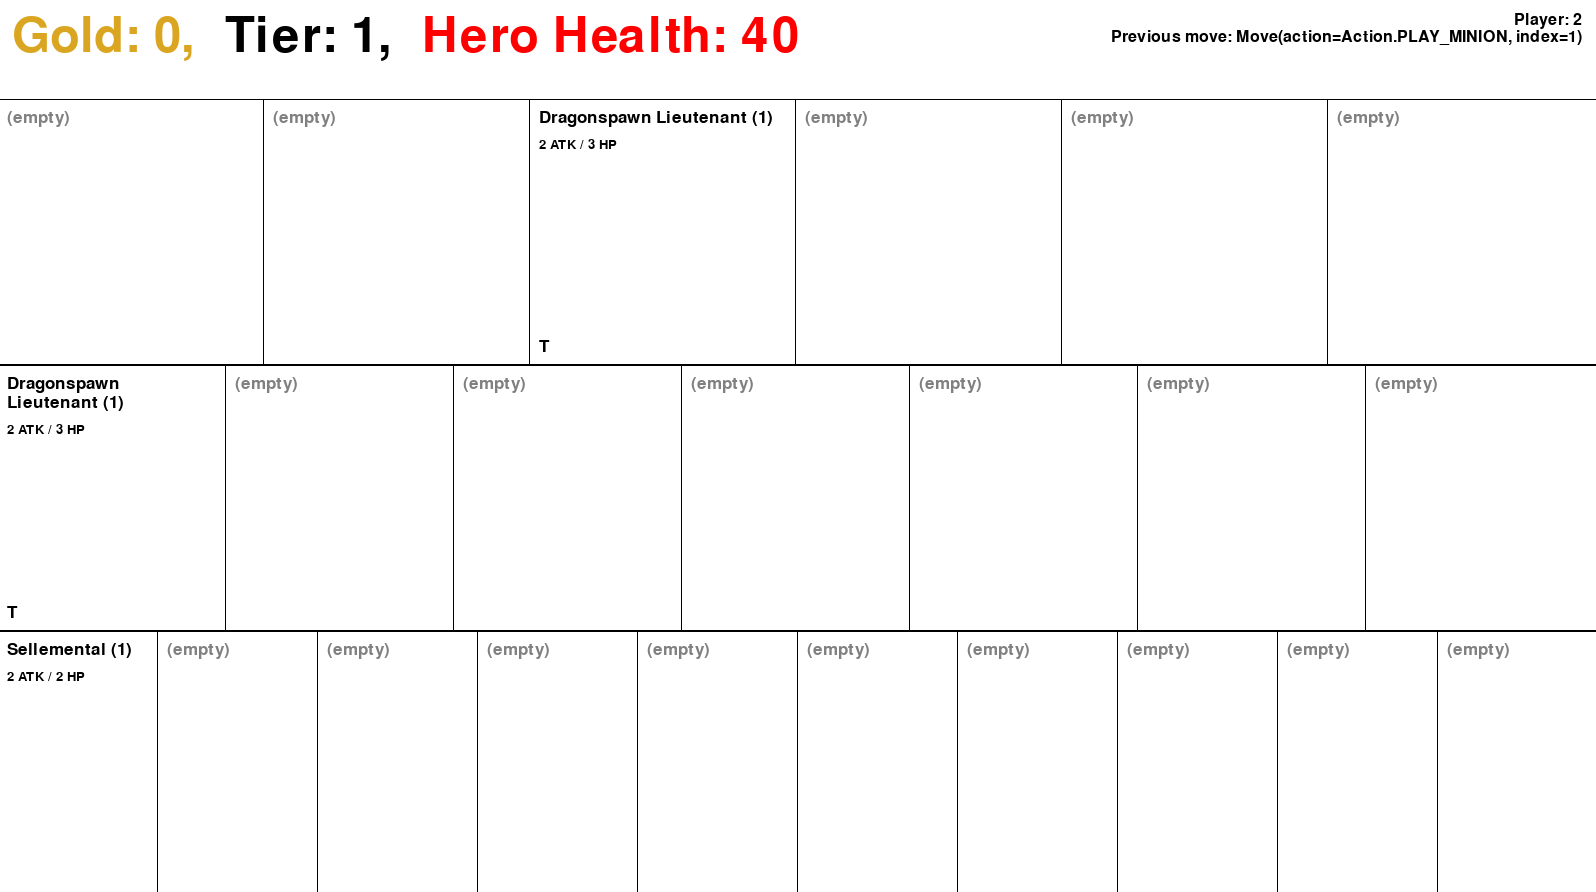
\includegraphics[width=0.8\textwidth]{figs/rudimentary board.png}}};
    
    % Gold
    \filldraw[draw=red!50!white,fill=red!20!white,opacity=1, fill opacity=0.25] (2,85) rectangle (20,75);
    
    \filldraw[draw=red!50!white,fill=red!20!white,] (2,85) rectangle (2+5, 85-5) node[color=black, text opacity=1,pos=0.5] {1};
    
    % Tier
    \filldraw[draw=red!50!white,fill=red!20!white,fill opacity=0.4, text opacity=1, fill opacity=0.25] (22,85) rectangle (40,75);
    
    \filldraw[draw=red!50!white,fill=red!20!white,] (22,85) rectangle (22+5,85-5) node[color=black,fill opacity=0.4, text opacity=1,pos=0.5] {2};
    
    % Hero Health
    \filldraw[draw=red!50!white,fill=red!20!white,opacity=1, fill opacity=0.25] (40,85) rectangle (82,75);
    
    \filldraw[draw=red!50!white,fill=red!20!white,] (40,85) rectangle (40+5,85-5) node[color=black,fill opacity=0.4, text opacity=1,pos=0.5] {3};
    
    % Recruits
    \filldraw[draw=red!50!white,fill=red!20!white,opacity=1, fill opacity=0.25] (2,75) rectangle (148,50);
    
    \filldraw[draw=red!50!white,fill=red!20!white,] (2,75)  rectangle (7,70) node[color=black,fill opacity=0.4, text opacity=1,pos=0.5] {4};
    
    % Board
    \filldraw[draw=red!50!white,fill=red!20!white,opacity=1, fill opacity=0.25] (2, 50) rectangle (148,26);
    
    \filldraw[draw=red!50!white,fill=red!20!white,]  (2, 50) rectangle  (2+5, 50-5) node[color=black,fill opacity=0.4, text opacity=1,pos=0.5] {5};
    
     % Board
    \filldraw[draw=red!50!white,fill=red!20!white,opacity=1, fill opacity=0.25] (2, 0) rectangle (148,26);
    
    \filldraw[draw=red!50!white,fill=red!20!white,]  (2, 26) rectangle  (7, 21) node[color=black,fill opacity=0.1, text opacity=1,pos=0.5] {6};
    
    \end{tikzpicture}
    \caption{Elements of the visualization of the Hearthstone game board during the recruitment phase: (1) gold, (2) tavern tier, (3) hero health, (4) the available recruits sold by Bob (5) your current board (6) your current hand. Each card on screen includes the name of the minion, the attack/health, and its special ability; minion abilities are shown on the bottom of the card, where the first letter of each ability (e.g. `T' for Taunt, `B' for Battlecry, and so on...) is used to denote the abilities. The top right also includes which player board is currently on screen, the previous move made. }
    \label{fig:rudimentaryboard}
    
\end{figure*}

\section{Differences from the Proposal}
Due to time constraints, we decided to leave out the Neural Network portion of our original computational plan out of the final project. Though, we did still include some modules that would've been used to implement the neural network in our final project, so feel free to check those files out. Other reasons for leaving out the Neural Network included that there was actually no need to train the bot anyways, since it performed surprisingly well without it. Removing the neural network portion also fixed the one issue the TA brought up on our proposal, but we have included more on implementing the neural network in our Further Works section later on!
\section{Experiments}
% - do the results of your computational exploration help answer the question
% - what limitations did you encouter, with the datasets you found, algorithm/libraries used, or other obstacles


After running the code and displaying with \texttt{plotly}, we found our results to be overall successful. 


\begin{figure*}[p]
    \centering
     \fbox{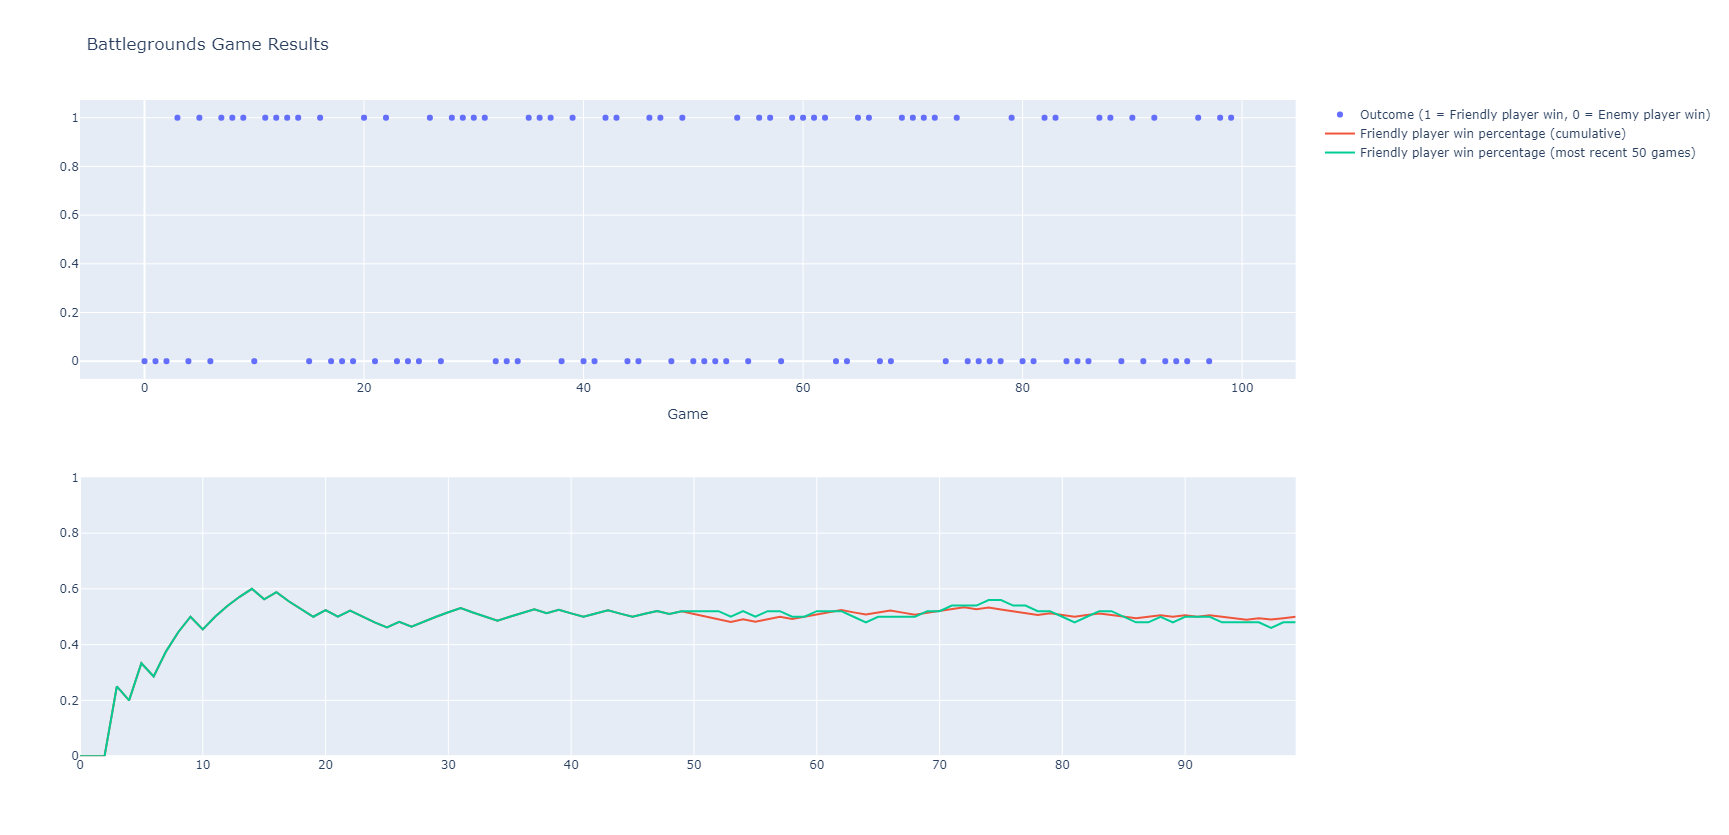
\includegraphics[width=0.7\textwidth]{figs/randomboi.png}}
     \caption{The graph for the outcome between two random players over 100 games.}
     \label{fig:exp1}
\end{figure*}
\begin{figure*}[p]
    \centering
     \fbox{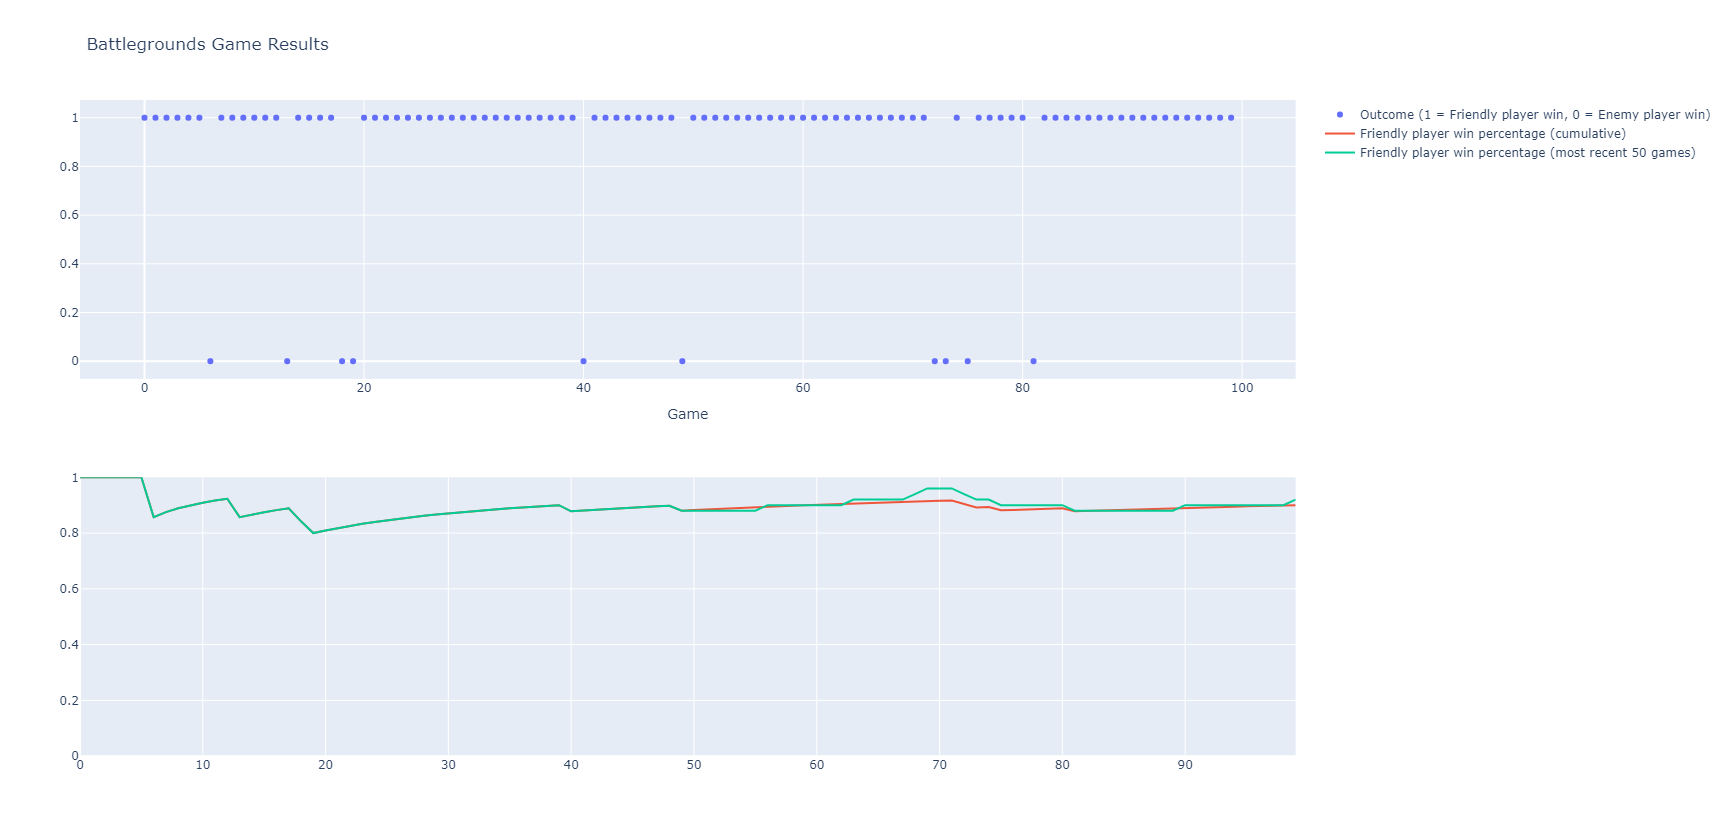
\includegraphics[width=0.7\textwidth]{figs/treeai.png}}
     \caption{The graph for the outcome between a tree player vs a random player over 100 games.}
     \label{fig:exp2}
\end{figure*}
\begin{figure*}[p]
    \centering
     \fbox{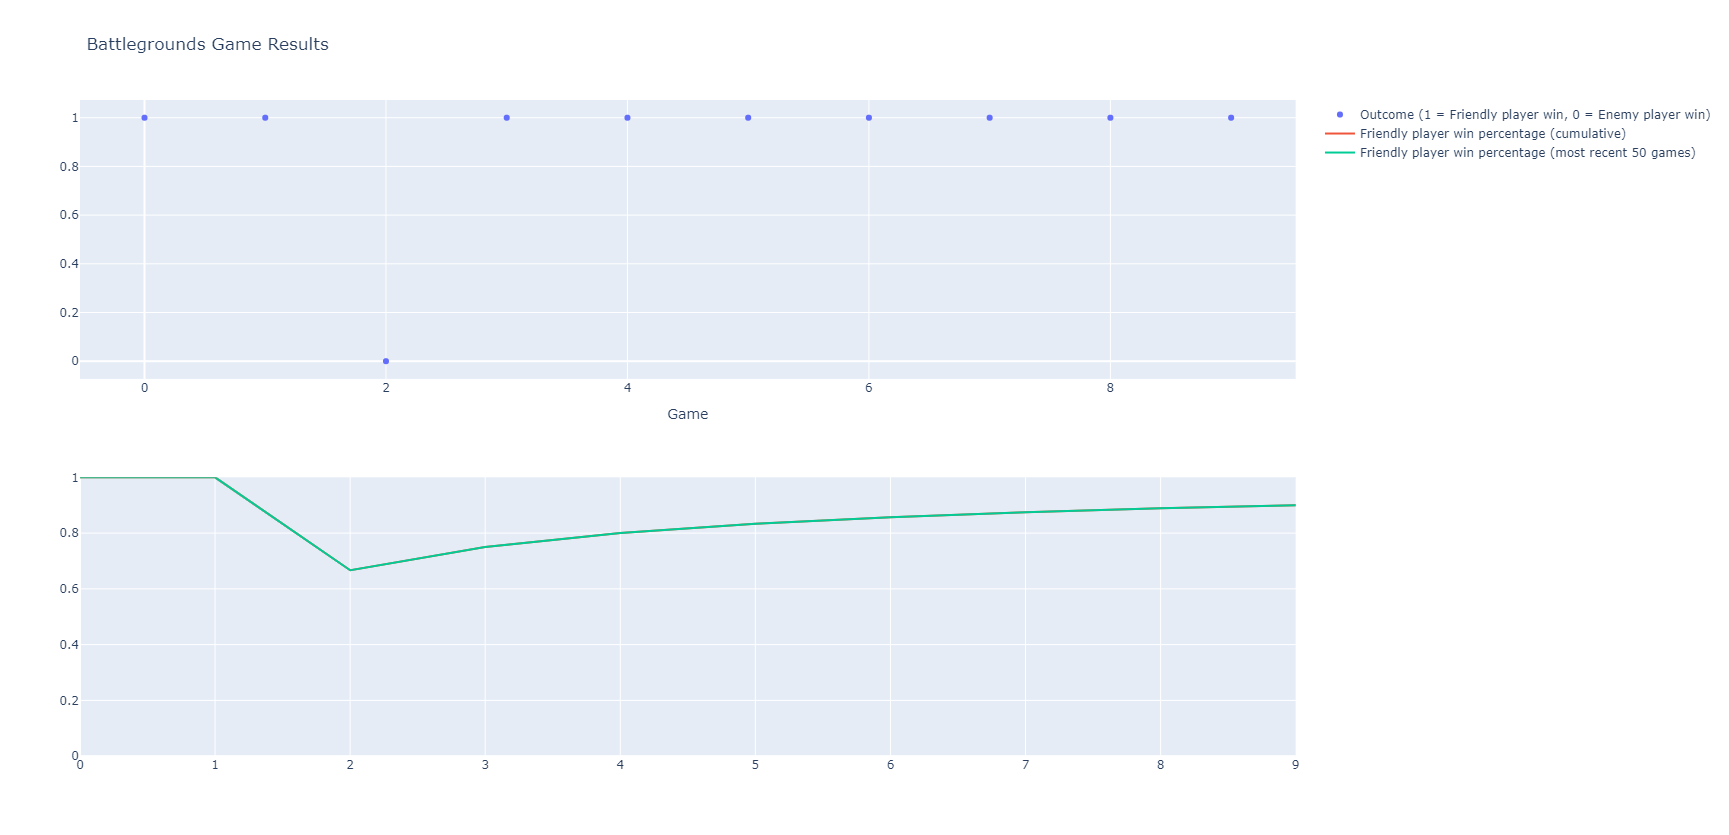
\includegraphics[width=0.7\textwidth]{figs/greedy.png}}
     \caption{The graph for the outcome between a greedy player vs a random player over 10 games.}
     \label{fig:exp3}
\end{figure*}

\inlineSection{Experiment 1 (Random Player vs Random Player)} In this experiment, we pitted two players that both uniformly randomly sample moves from the action space against each other. This experiment provided a helpful baseline for the rest of the experiments, and was helpful in testing the code for the simulator. It also gave us a goal to beat for our other players. The results of the experiment were as expected: each player always wins roughly \textit{half} of all games, which agrees with intuition and statistics theory (each player is just as likely to win). See Figure \ref{fig:exp1} for the cumulative and total win rates for this experiment. Pretty basic, but we're off to a good start! 

\inlineSection{Experiment 2 (MCTS Player vs Random Player)} In this experiment, we put a player using the MCTS algorithm against a player that moves randomly. This is where things got interesting! Though we expected the MCTS player to do well, we were surprised by the results as they exceeded our expectations. On average, the MCTS player wins 80 to 100\% of all games. See Figure \ref{fig:exp2} for the cumulative and total win rates for this experiment. This is particularly impressive considering the fact that no pre-training is performed on our player.  The MCTS player is only training as it plays the game.

\inlineSection{Experiment 3 (Greedy Player vs Random Player)} The next experiment we did pitted a random player against a greedy player, which will always choose the move that maximizes average reward (state value). In many ways, the greedy player is a naive implementation of the MCTS player---they are both fundamentally based on the same idea: evaluate possible future states to find the best move now. As a result, just like the MCTS player, the greedy player performed exceptionally well against the random player, winning against it almost every single round. See Figure \ref{fig:exp3} for the cumulative and total win rates for this experiment. However, the greedy player takes an obscenely long time to run as it simulates a fixed number of games \textit{for every} possible move \textit{for every} state of the game. In this represents the inherent advantage of using the MCTS algorithm: iterative rollouts and heuristics like UCT mean that we don't waste time evaluating `useless' states. Though we did not evaluate the greed player for a large set of games, we are confident that it would maintain the trend we observed. Nonetheless, evaluating the greedy player on a larger set of games is still desired.

\inlineSection{Conclusion} Overall, outside some time issues, our program ran fairly well, showing that it is possible to create an AI agent to play Hearthstone Battlegrounds! Though, there are some further things we would like to work on, given more time to do the project. 

\section{Further Work}
Originally in our project proposal, we wanted to use an agent policy estimation and deep neural network to train the AI. Though that is not included in our program, we do still have some rough work from when we were working on it, so we thought it would be nice to include an explanation of our future plans. 

This section details further improvements that could be made to our approach, but ones which we did not end up implementing.\footnote{Due to time and computational constraints.}

\subsection{Policy Estimation with Deep Neural Networks}\label{sec:policy_estimation}
An agent policy governs how it behaves at any given state of the game. We would train a deep neural network to predict the state-value---a measure of how good the state is from the perspective of the current player---and agent policy of a given game state. Training would be done in an unsupervised manner through \textit{self-play}. In self-play, the agent plays against itself and previous games are used as training data for the policy network. At the beginning, both agents would make completely random actions; however, the hope is that over time, the network would converge to a local minimum (with respect to the loss function) and in the process learn which states \textit{eventually} lead to wins. Meanwhile, sampling the learned policy should give a reasonable estimate for which actions are best from any given state.

More formally, the `agent function' $\mathcal{F}$---that is, the agent's policy---would first be estimated using a neural network. In training, the network would be provided examples of the form $(s_t,\pi_t,z_t)$ where $s_t$ is the state at the $t$-th timestep, $\pi_t$ is an estimate of the policy from state $s_t$, and $z_t\in\{-1,1\}$ is a dummy variable indicating the final outcome of the game ($+1$ if the player wins, and $-1$ if the player loses). The value of $z_t$ is analogous to the result of a single simulation step in MCTS ($z_t$ is the outcome of the game if we continue from state $s_t$, which is what the simulation phase computes). The network is trained to minimize the sum of deviations between the ground truth outcome $z_t$ and the estimated state-value $V^\pi(S)$ over all timesteps.

The neural network would be implemented and trained with the TensorFlow Python package. In specific, TensorFlow provides an interface for performing fast mathematical operations (such as matrix multiplication,  which is core to training a deep neural  network) on the GPU \cite{tensorflow2015-whitepaper}. It includes the \texttt{tf.keras} which simplifies the process of defining neural networks by providing common implementations of common layers and activations functions such as 2D convolutional layers (\texttt{tf.keras.layers.Conv2D}), fully connected/linear layers (\texttt{tf.keras.layers.Dense}), ReLU activation (\texttt{tf.keras.activations.relu}), softmax activation (\texttt{tf.keras.activations.softmax}), and more \cite{tf_keras_docs}. 

\subsection{Augmenting MCTS with the Policy Estimator}
Performing rollout is computationally expensive since it requires simulating an entire game until completion. Even with our fast simulator implementation, training a Monte Carlo Tree Searcher is computationally expensive (and this grows with the number of rollouts that we do per move!).

Following an approach by Silver, et. al. in their \textit{AlphaGo Zero} implementation, we would leverage the policy-estimation network described in Section \ref{sec:policy_estimation} to predict the game outcome from a given state \cite{Silver2017}. Recall that $\mathcal{F}$ provides along with the estimated policy, an estimate of the state-value, which is a measure of how favourable the state is from the perspective of the current player. During the rollout phase, we would obtain the state-value from the network and then propagate it up the tree \cite{alpha_zero}. The state-value predicted by $\mathcal{F}$ acts as a replacement for the simulation step of MCTS. Then, during model training (i.e. self-play), we would perform a fixed number of MCTS simulations from the current state. This gives us an improved policy from which we can use to sample actions.

\subsection{Card Vectorization}

We may further augment the neural network training process by training a model to convert Hearthstone cards into an efficient vector representation. This would allow for a more efficient game-state representation, which would improve training of the neural network.

Most Hearthstone cards have a textual description of its function. Thus, we can use a word embeddings model, such as \textit{word2vec}, to learn embeddings from cards' textual description. First, we would train a word2vec model on the Hearthstone wiki data. This would produce a word embedding model $\mathcal{W}$ that is trained on \textit{Hearthstone vocabulary}. The intuition is that a model trained on the Hearthstone wiki will be able to better capture the meaning of words as they relate to the game. It also has the benefit of including words exclusive to Hearthstone such as Murloc, and Windfury (which we would have to augment if we were using a model trained on a more general dataset).

Using the word2vec model, we can produce an embedding vector for a specific card by aggregating the individual vectors of its textual description. In specific, there are five feature vectors that are summed together to make the card embedding: Each feature vector describes an attribute of the minion: text description, race/minion type, tavern tier, attack, and health. They are computed as follows
\begin{enumerate}
    \item \textbf{text}: the average of the word embedding vectors for the text description of the card.
    \item \textbf{race/minion type}: the word embedding vector corresponding to the minion type (e.g. `murloc', `demon', etc...). So, the feature vector $\vec{v}(d)$ for a card description $d$ represented as a set of words is given by $$\displaystyle\vec{v}(d)=\frac{1}{|d|}\sum_{w\in d}\mathcal{W}(d).$$
    \item \textbf{tavern tier}: the element-wise product between the word embedding vector for ``tier'' and the word embedding vector for the text representation of the tavern tier of the card (i.e. ``one``, ``two,`` etc...). So, the feature vector $\vec{v}(t)$ for a card tavern tier $t$ is given by $$\displaystyle\vec{v}(t)=\mathcal{W}(\text{tier}) \odot \mathcal{W}(t),$$ where it is assumed that $\mathcal{W}(t)$ gives the embedding vector for the word representing the numerical value of $t$.
    
    \item \textbf{attack}: the element-wise product between the word embedding vector for ``attack'' and the word embedding vector for the text representation of the attack of the card (i.e. ``one``, ``two,`` etc...). So, the feature vector $\vec{v}(t)$ for a card attack $a$ is given by $$\displaystyle\vec{v}(a)=\mathcal{W}(\text{attack}) \odot \mathcal{W}(a),$$ where it is assumed that $\mathcal{W}(a)$ gives the embedding vector for the word representing the numerical value of $a$.
    
    \item \textbf{health}: the element-wise product between the word embedding vector for ``health'' and the word embedding vector for the text representation of the health of the card (i.e. ``one``, ``two,`` etc...). So, the feature vector $\vec{v}(t)$ for a card health $h$ is given by $$\displaystyle\vec{v}(h)=\mathcal{W}(\text{health}) \odot \mathcal{W}(h),$$ where it is assumed that $\mathcal{W}(a)$ gives the embedding vector for the word representing the numerical value of $h$.
    
\end{enumerate}
Let $X\in\mathcal{C}$ be a card, where $\mathcal{C}$ is the set of all cards. Then, the embedding vector for $X$ is given as
\begin{equation*}
    \mathcal{E}(X)=\frac{1}{|f(X)|}\sum_{\vec{v}\in{f}(X)}\vec{v},
\end{equation*}
where $f(X)$ is the set of feature vectors for card $X$ (computed according to the description above).

\section{Conclusion}
Though the Battlegrounds domain is fairly complex, we were able to successfully implement an efficient agent using the Monte-Carlo Tree Search Algorithm, and compare its abilities against a random player. In the future, there are possible room for improvements, including experimenting with a user player. However, with what we have implemented now, it is to answer our research question, and give us the desired results.

% Start references
\FloatBarrier
\clearpage
\printbibliography[]


\end{document}
